\section{Geschichte und Einführung}

\subsection{Geschichte}

\begin{enumerate}
    \item Lambda Kalkül
        \begin{itemize}
            \item Gleichwertig mit Turing Maschine (kann gleichen Probleme lösen)
            \item Universale Turing Maschine (kann alle Turingmaschinen beschreiben)
            \item Universale Lambda-Funktion gesucht
        \end{itemize}

    \item Fortran (Fortran list processing language)

    \item Fortran M-Expressions (Idee wurde nie implementiert)

    \item Lisp
        \begin{itemize}
            \item List processing Alternative zu Turingmaschine: LISP Funktion eval
            \item Notation: Programme und Daten können beide als Liste beschrieben werden
                \begin{figure}[h!]
                	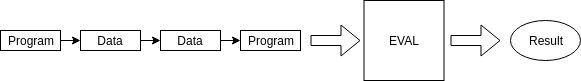
\includegraphics[width=\linewidth]{pics/lisp-notation}
                	\caption{LISP EVAL vereinfacht}
                \end{figure}
            \item EVAL ist LISP Interpreter
        \end{itemize}

    \item Scheme
        \begin{itemize}
            \item Prototyp für funktionale Programmiersprache
            \item Versuch, LISP simpler umzusetzen
            \item Optimized tail recursion (garantiert vom Compiler)
        \end{itemize}
\end{enumerate}

\subsection{Tail call optimization}
Tailcall Rekursion ist fast so effizient wie \textbf{goto} Begehle weil keine neuen
Stackframes aufgebaut werden müssen.

\subsubsection{Tail recursion}
Rekursive Funktion f ist \textbf{endrekursiv}, wenn der rekursive Funktionsaufruf die \textbf{letzte Aktion zur Berechnung von f} ist.

\subsubsection{Beispiele}
\lstset{language=C,style=customstyle}
\begin{lstlisting}
// Kein tail call
int fact(int x){
    if(x == 0) return 1;
    else return fact(x - 1) * x;
}
\end{lstlisting}


\lstset{language=C,style=customstyle}
\begin{lstlisting}
// Tail call
int fact(int x, int accum=1){
    if(x == 0) return accum;
    else return fact(x - 1, x * accum);
}
\end{lstlisting}
\textbf{\textit{Optimierung möglich, da x nicht als Zwischenergebnis gespeichert werden muss.}}
